
\chapter{Введение}

\section{Актуальность темы исследования}

Беспилотные летательные аппараты (БЛА) мультироторного типа находят всё более широкое применение в различных областях человеческой деятельности, а миниатюризация и доступность электронных компонентов их бортового оборудования приводит к расширению спектра задач, в решении которых используются такие аппараты.
Интерес исследователей к БЛА обусловлен также и тем, что они являются доступным средством для отработки новых технологий в аэрокосмической отрасли \cite{Otero01}.
С момента создания первых квадрокоптеров интенсивно ведутся исследования в области их динамики и управления, причём количество работ растет с каждым годом, что можно наблюдать по динамике количесва публикаций, посвященных квадрокоптерам, доступных на крупнейшей онлайн платформе научных публикаций «Google Академия».
Однако, несмотря на обилие публикаций, в области управляемой динамики квадрокоптеров остаются перспективные направления, среди которых усовершенствование конструкции БЛА, связанное с увеличением размерности вектора управляющих воздействий.
Конструктивно это достигается, например, с помощью сервоприводов, способных поворачивать роторы с пропеллерами относительно корпуса.
\begin{figure}[h!]
	\centering
	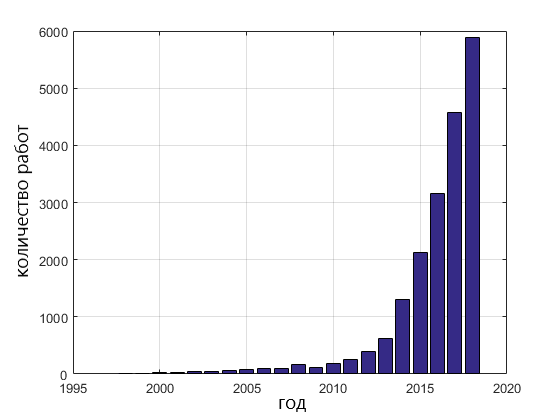
\includegraphics[width=0.95\columnwidth]{res_amount}
	\label{res_amount}
\end{figure}

Стандартный квадрокоптер с четырёхмерным вектором управляющих воздействий и шестью степенями свободы корпуса аппарата не способен, например, независимо управлять положением и ориентацией.
Это приводит к необходимости дополнительных устройств для наведения камер или лазерных дальномеров, используемых при выполнении ряда стандартных для БЛА задач.
Возможность независимо управлять положением и ориентацией, приобретаемая за счёт использования поворотных роторов, влияет не только на работу полезной нагрузки и датчиков, но и на функциональные возможности всей системы в целом.
Согласно работе \cite{Stolc01} усовершенствованные таким образом квадрокоптеры более устойчивы к возмущениям внешней среды, а также лучше стандартных квадрокоптеров пригодны для вертикального взлёта и посадки на неровные поверхности.
Достоинства БЛА с поворотными роторами отмечают и исследователи, работающие над управлением БЛА в экстренных ситуациях (при отказе части двигателей) \cite{Morozov01, Shidar00}.
В работе \cite{Shidar00} обосновывается достижение более высокой скорости за счёт выбора оптимальной по отношению к набегающему потоку ориентации, а также более рациональное по сравнению со стандартными аппаратами энергопотребление.
В работе \cite{Morozov01} отмечена перспективность конструкции с поворотными роторами, однако её применение не рассматривается из-за сложности реализации.
Использование поворотных роторов действительно усложняет реализацию контура управления \cite{Ryll01, Falconi01, Segui01, Oosedo01} и не позволяет применять ставшую классической изящную схему управления \cite{Mellinger01}, однако, есть основания полагать, что предлагаемое в данной работе аналитическое обращение динамики системы позволит преодолеть некоторую часть возникающих трудностей.

\section{Цели и задачи исследования}

Цель работы - синтезировать систему управления квадрокоптером с поворотными роторами с использованием дополнительных степеней свободы для достижения независмого управления по всем шести степеням свободы.

Для достижения поставленной цели были поставлены и решены
следующие задачи:
\begin{enumerate}
	\item Разработать математической модели динамики БЛА с поворотными роторами.
	\item Синтезировать регулятор и обратить динамику модели.
	\item Ввести ограничения на компоненты вектора управляющих воздействий.
	\item Реализовать обратные связи в контуре управления.
\end{enumerate}

\section{Научная новизна и практическая значимость работы}
Получены аналитическое обращение динамики квадрокоптера с поворотными роторами а также введены ограничения на компоненты вектора управляющих воздействий.

\section{Методология и методы исследования}

\section{Положения, выносимые на защиту}

\section{Степень достоверности и апробация результатов}
По теме диссертации опубликованы следующие работы: (В СПИСКЕ В КОНЦЕ)

